\begin{pastexam}[label={px:gw3-108-ds-03}]{關務三等資訊處理 108 年 第三題}
（申論；30 分）

給定以相鄰矩陣（adjacency matrix）表示的圖 G，矩陣中的數字為相鄰兩節點間的距離，若空白則代表兩節點不相鄰。
\begin{center}
\begin{tabular}{|c|*{9}{c|}}
\hline
G & a & b & c & d & e & f & g & h & j \\
\hline
a & & 1 & 6 & 5 & & & & & \\
\hline
b & 1 & & 6 & & & & & & \\
\hline
c & 6 & 6 & & & 7 & 3 & & & \\
\hline
d & 5 & & & & & 2 & 10 & & \\
\hline
e & & & 7 & & & & & 12 & \\
\hline
f & & & 3 & 2 & & & & 8 & \\
\hline
g & & & & 10 & & & & 7 & 3 \\
\hline
h & & & & & 12 & 8 & 7 & & 8 \\
\hline
j & & & & & & & 3 & 8 & \\
\hline
\end{tabular}\\[0.3em]
圖G
\end{center}
\begin{enumerate}[leftmargin=2.2em]
\item[㈠] 請說明若以 Kruskal's 演算法建立最小生成樹（minimum spanning tree）的過程中，依序被加入生成樹的邊。（5 分）
\item[㈡] 請說明若以 Prim's 演算法建立最小生成樹（minimum spanning tree）的過程中，依序被加入生成樹的邊。（5 分）
\item[㈢] 請說明 Dijkstra's 演算法的用途，並說明該演算法應用上的限制。（10 分）
\item[㈣] 請說明將圖 G 從 f 節點開始執行 Dijkstra's 演算法的過程並顯示節點加入的順序。（10 分）
\end{enumerate}
\end{pastexam}

\begin{pastsoln}
四個小題中 ㈠ ㈡ 屬資結書第~24~章，㈢ ㈣ 屬第~25~章，配分較重的最短路徑放在這一章。 矩陣是對稱的，
G 是無向圖，有 9 個節點、13 條邊：
\begin{center}
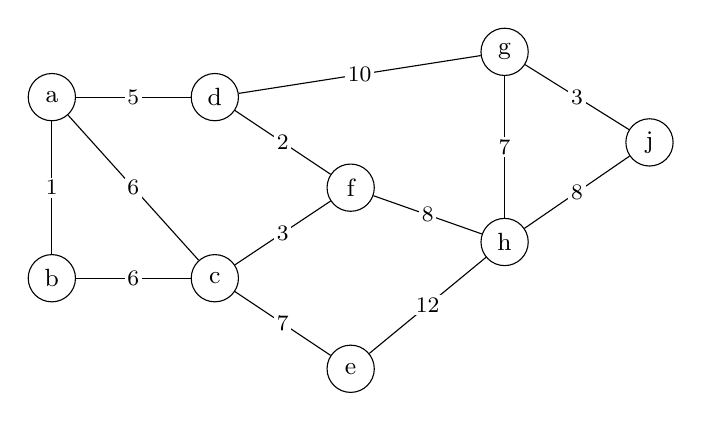
\begin{tikzpicture}[x=1.15cm, y=1.15cm,
    v/.style={circle, draw, minimum size=6mm, inner sep=0pt, font=\small},
    w/.style={fill=white, inner sep=1pt, font=\footnotesize}]
\node[v] (a) at (0,1) {a};
\node[v] (b) at (0,-1) {b};
\node[v] (c) at (1.8,-1) {c};
\node[v] (d) at (1.8,1) {d};
\node[v] (f) at (3.3,0) {f};
\node[v] (e) at (3.3,-2) {e};
\node[v] (g) at (5,1.5) {g};
\node[v] (h) at (5,-0.6) {h};
\node[v] (j) at (6.6,0.5) {j};
\draw (a) -- node[w] {1} (b);
\draw (a) -- node[w] {6} (c);
\draw (a) -- node[w] {5} (d);
\draw (b) -- node[w] {6} (c);
\draw (c) -- node[w] {7} (e);
\draw (c) -- node[w] {3} (f);
\draw (d) -- node[w] {2} (f);
\draw (d) -- node[w] {10} (g);
\draw (e) -- node[w] {12} (h);
\draw (f) -- node[w] {8} (h);
\draw (g) -- node[w] {7} (h);
\draw (g) -- node[w] {3} (j);
\draw (h) -- node[w] {8} (j);
\end{tikzpicture}
\end{center}

\textbf{㈠ Kruskal。} 邊由輕到重：a-b 1；d-f 2；c-f 3、g-j 3；a-d 5；a-c 6、b-c 6；c-e 7、g-h 7；f-h 8、h-j 8；
d-g 10；e-h 12。 依序檢查，會成環就丟掉（資結書第~24.2~節）：
\begin{center}
\begin{tabular}{cll}
\toprule
邊 & 結果 & 加入後的元件 \\
\midrule
a-b 1 & 加入 & \{a,b\} \\
d-f 2 & 加入 & \{a,b\} \{d,f\} \\
c-f 3 & 加入 & \{a,b\} \{c,d,f\} \\
g-j 3 & 加入 & \{a,b\} \{c,d,f\} \{g,j\} \\
a-d 5 & 加入 & \{a,b,c,d,f\} \{g,j\} \\
a-c 6 & 丟掉（a、c 已連通） & \\
b-c 6 & 丟掉 & \\
c-e 7 & 加入 & \{a,b,c,d,e,f\} \{g,j\} \\
g-h 7 & 加入 & \{a,b,c,d,e,f\} \{g,h,j\} \\
f-h 8 & 加入 & 全部 9 個節點，8 條邊，停止 \\
\bottomrule
\end{tabular}
\end{center}
依序加入：(a,b)、(d,f)、(c,f)、(g,j)、(a,d)、(c,e)、(g,h)、(f,h)，總權重 $1+2+3+3+5+7+7+8 = 36$。 權重相同的
邊（c-f 與 g-j、c-e 與 g-h、f-h 與 h-j）先後次序不影響結果：前兩組兩條都會加入；h-j 不論排在 f-h 前或後，
那時 h、j 都已經經由 g 連在一起，都會被丟掉。

\textbf{㈡ Prim。} 題目沒有指定起點，這裡從 a 開始（資結書第~24.3~節）。 每一步選「一端在樹裡、一端不在」
最輕的邊，括號是樹外節點目前最輕的連接邊：
\begin{center}
\begin{tabular}{cll}
\toprule
步 & 樹外節點的最輕連接邊 & 加入 \\
\midrule
1 & b:1(a), c:6(a), d:5(a) & (a,b) 1 \\
2 & c:6(a 或 b), d:5(a) & (a,d) 5 \\
3 & c:6(a), f:2(d), g:10(d) & (d,f) 2 \\
4 & c:3(f), g:10(d), h:8(f) & (f,c) 3 \\
5 & e:7(c), g:10(d), h:8(f) & (c,e) 7 \\
6 & g:10(d), h:8(f) & (f,h) 8 \\
7 & g:7(h), j:8(h) & (h,g) 7 \\
8 & j:3(g) & (g,j) 3 \\
\bottomrule
\end{tabular}
\end{center}
依序加入：(a,b)、(a,d)、(d,f)、(f,c)、(c,e)、(f,h)、(h,g)、(g,j)，總權重 36，和 Kruskal 選的是同一組邊。

\textbf{㈢ 用途與限制。}
\begin{itemize}
\item \textbf{用途}：單源最短路徑。 給一張邊上有權重（距離、時間、成本）的有向或無向圖和一個起點 $s$，
求 $s$ 到每個節點的最短距離和最短路徑，例如導航、網路路由（OSPF 用的就是它）。 做法是每次從還沒確定的
節點中取出目前距離最小的、確定它，再用它放鬆相鄰的邊（資結書第~25.2~節）。 只要某一個終點，取出該點時就
可以提早停止。
\item \textbf{限制}：
\begin{enumerate}
\item \textbf{邊權不能是負的。} 演算法的正確性靠「被取出的節點距離已經最短」，這要求之後經過的邊不會讓
距離變小。 有負邊時可能先確定了某點，之後才發現經過負邊的更短路徑，答案就錯了（資結書第~25.2.5~節）。
例如 $s \to u$ 權 2、$s \to v$ 權 3、$v \to u$ 權 $-2$：Dijkstra 先確定 $u$ 的距離 2，但真正最短是
$3 - 2 = 1$。 有負邊要改用 Bellman-Ford；有負環則最短路徑沒有定義。
\item 只解單一起點；要所有點對時要對每個起點各跑一次，或改用 Floyd-Warshall。
\item 時間 $O(|V|^2)$（陣列）或 $O((|V|+|E|)\log|V|)$（二元堆積），圖很大時需要好的優先佇列。
\end{enumerate}
\end{itemize}

\textbf{㈣ 從 f 開始。} $d[\cdot]$ 是目前的距離估計，粗體是這一步被取出（確定）的節點；距離相同時取字母順序
在前的。
\begin{center}
\small
\begin{tabular}{cc*{8}{c}}
\toprule
步 & 取出 & a & b & c & d & e & g & h & j \\
\midrule
0 & f (0) & $\infty$ & $\infty$ & 3 & 2 & $\infty$ & $\infty$ & 8 & $\infty$ \\
1 & d (2) & 7 & $\infty$ & 3 & \textbf{2} & $\infty$ & 12 & 8 & $\infty$ \\
2 & c (3) & 7 & 9 & \textbf{3} & & 10 & 12 & 8 & $\infty$ \\
3 & a (7) & \textbf{7} & 8 & & & 10 & 12 & 8 & $\infty$ \\
4 & b (8) & & \textbf{8} & & & 10 & 12 & 8 & $\infty$ \\
5 & h (8) & & & & & 10 & 12 & \textbf{8} & 16 \\
6 & e (10) & & & & & \textbf{10} & 12 & & 16 \\
7 & g (12) & & & & & & \textbf{12} & & 15 \\
8 & j (15) & & & & & & & & \textbf{15} \\
\bottomrule
\end{tabular}
\end{center}
每一列是取出該節點、放鬆它的邊之後的值：
\begin{itemize}
\item 取 f：c $= 3$、d $= 2$、h $= 8$。
\item 取 d (2)：a $= 2+5 = 7$，g $= 2+10 = 12$。
\item 取 c (3)：a 經 c 是 $3+6 = 9 > 7$ 不變；b $= 3+6 = 9$；e $= 3+7 = 10$。
\item 取 a (7)：b 經 a 是 $7+1 = 8 < 9$，改成 8。
\item b、h 都是 8，取 b：鄰居 a、c 都已確定。 再取 h (8)：e 經 h 是 20，不變；g 經 h 是 15，不變；j $= 8+8 = 16$。
\item 取 e (10)：沒有可改的。 取 g (12)：j 經 g 是 $12+3 = 15 < 16$，改成 15。 最後取 j (15)。
\end{itemize}
節點加入的順序：\textbf{f, d, c, a, b, h, e, g, j}（b、h 同為 8，先取哪個都可以）。 最短距離與路徑：
\begin{center}
\begin{tabular}{cccccccc}
\toprule
a & b & c & d & e & g & h & j \\
\midrule
7 & 8 & 3 & 2 & 10 & 12 & 8 & 15 \\
f-d-a & f-d-a-b & f-c & f-d & f-c-e & f-d-g & f-h & f-d-g-j \\
\bottomrule
\end{tabular}
\end{center}
\end{pastsoln}
